\begin{figure}[H]
    \centering
    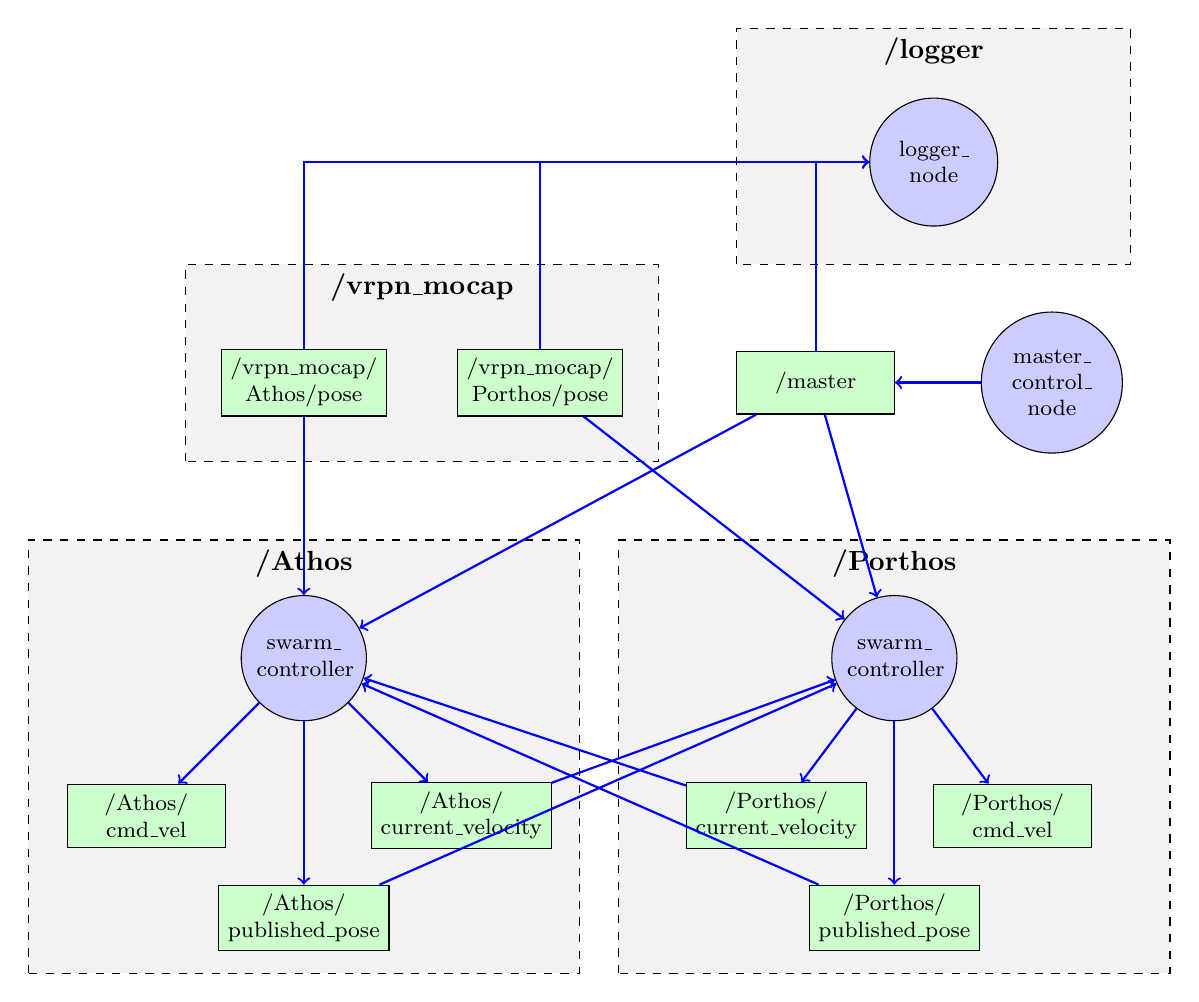
\begin{tikzpicture}[
        node/.style={circle, draw, fill=blue!20, minimum size=1.5cm, text width=1.2cm, align=center, font=\footnotesize},
        topic/.style={rectangle, draw, fill=green!20, minimum width=2cm, minimum height=0.8cm, align=center, font=\footnotesize},
        namespace/.style={rectangle, draw, dashed, fill=gray!10, minimum width=3cm, minimum height=2cm},
        arrow/.style={->, thick, blue}
    ]
    
    % Namespace /vrpn_mocap (décalé à gauche)
    \draw[namespace] (-1, 5) rectangle (5, 7.5);
    \node at (2, 7.2) {\textbf{/vrpn\_mocap}};
    
    % Topics dans /vrpn_mocap
    \node[topic] (athos_pose) at (0.5, 6) {/vrpn\_mocap/\\Athos/pose};
    \node[topic] (porthos_pose) at (3.5, 6) {/vrpn\_mocap/\\Porthos/pose};
    
    % Namespace /Athos (adapté en hauteur)
    \draw[namespace] (-3, -1.5) rectangle (4, 4);
    \node at (0.5, 3.7) {\textbf{/Athos}};
    
    % Namespace /Porthos (adapté en hauteur)
    \draw[namespace] (4.5, -1.5) rectangle (11.5, 4);
    \node at (8, 3.7) {\textbf{/Porthos}};
    
    % Nodes swarm_controller
    \node[node] (swarm_athos) at (0.5, 2.5) {swarm\_\\controller};
    \node[node] (swarm_porthos) at (8, 2.5) {swarm\_\\controller};
    
    % Topics cmd_vel (descendus)
    \node[topic] (athos_cmd) at (-1.5, 0.5) {/Athos/\\cmd\_vel};
    \node[topic] (porthos_cmd) at (9.5, 0.5) {/Porthos/\\cmd\_vel};
    
    % Topics published_pose (descendus)
    \node[topic] (athos_pub_pose) at (0.5, -0.8) {/Athos/\\published\_pose};
    \node[topic] (porthos_pub_pose) at (8, -0.8) {/Porthos/\\published\_pose};
    
    % Topics current_velocity (descendus)
    \node[topic] (athos_curr_vel) at (2.5, 0.5) {/Athos/\\current\_velocity};
    \node[topic] (porthos_curr_vel) at (6.5, 0.5) {/Porthos/\\current\_velocity};
    
    % Topic /master (ajusté)
    \node[topic] (master_topic) at (7, 6) {/master};
    
    % Node master_control_node (ajusté)
    \node[node] (master_node) at (10, 6) {master\_\\control\_\\node};
    
    % Namespace /logger (ajusté en taille)
    \draw[namespace] (6, 7.5) rectangle (11, 10.5);
    \node at (8.5, 10.2) {\textbf{/logger}};
    
    % Node logger (légèrement remonté)
    \node[node] (logger_node) at (8.5, 8.8) {logger\_\\node};
    
    % Arrows - subscriptions
    \draw[arrow] (athos_pose) -- (swarm_athos);
    \draw[arrow] (porthos_pose) -- (swarm_porthos);
    \draw[arrow] (master_topic) -- (swarm_athos);
    \draw[arrow] (master_topic) -- (swarm_porthos);
    
    % Logger subscriptions (nouvelles)
    \draw[arrow] (athos_pose) |- (logger_node);
    \draw[arrow] (porthos_pose) |- (logger_node);
    \draw[arrow] (master_topic) |- (logger_node);
    
    % Cross-subscriptions entre robots
    \draw[arrow] (porthos_pub_pose) -- (swarm_athos);
    \draw[arrow] (porthos_curr_vel) -- (swarm_athos);
    \draw[arrow] (athos_pub_pose) -- (swarm_porthos);
    \draw[arrow] (athos_curr_vel) -- (swarm_porthos);
    
    % Arrows - publications cmd_vel
    \draw[arrow] (swarm_athos) -> (athos_cmd);
    \draw[arrow] (swarm_porthos) -> (porthos_cmd);
    
    % Publications des nouveaux topics
    \draw[arrow] (swarm_athos) -> (athos_pub_pose);
    \draw[arrow] (swarm_athos) -> (athos_curr_vel);
    \draw[arrow] (swarm_porthos) -> (porthos_pub_pose);
    \draw[arrow] (swarm_porthos) -> (porthos_curr_vel);
    
    % Arrow - publication master
    \draw[arrow] (master_node) -- (master_topic);
    
    \end{tikzpicture}
    \caption{Organisation simplifiée du système ROS2 pour la méthode prédictive}
    \label{fig:ros2_system}
    \end{figure}